\def\iangle{35} % Angle of the inclined plane

\def\down{-90}
\def\arcr{0.5cm} % Radius of the arc used to indicate angles

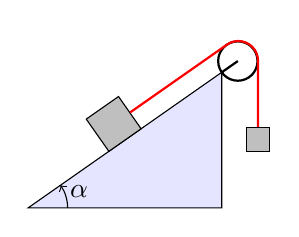
\begin{tikzpicture}[
    force/.style={>=latex,draw=blue,fill=blue},
    axis/.style={densely dashed,gray,font=\small},
    M/.style={rectangle,draw,fill=lightgray,minimum size=0.5cm,thin},
    m/.style={rectangle,draw=black,fill=lightgray,minimum size=0.3cm,thin},
    plane/.style={draw=black,fill=blue!10},
    string/.style={draw=red, thick},
    pulley/.style={thick},
]

\draw[plane] (0,-1) coordinate (base)
                 -- coordinate[pos=0.5] (mid) ++(\iangle:3) coordinate (top)
                 |- (base) -- cycle;
\path (mid) node[M,rotate=\iangle,yshift=0.25cm] (M) {};
\draw[pulley] (top) -- ++(\iangle:0.25) circle (0.25cm)
               ++ (90-\iangle:0.5) coordinate (pulley);
\draw[string] (M.east) -- ++(\iangle:1.5cm) arc (90+\iangle:0:0.25)
              -- ++(0,-1) node[m] {};

\draw[->] (base)++(\arcr,0) arc (0:\iangle:\arcr);
\path (base)++(\iangle*0.5:\arcr+5pt) node {$\alpha$};

\end{tikzpicture}

\begin{tikzpicture}[
    force/.style={>=latex,draw=blue,fill=blue},
    M/.style={rectangle,draw,fill=lightgray,minimum size=0.5cm,thin},
    m/.style={rectangle,draw=black,fill=lightgray,minimum size=0.3cm,thin},
    string/.style={draw,thick},
    pulley/.style={thick},
    obj/.style={rectangle,draw,minimum size=0.2cm,fill=blue!10},
]

\path (mid) node[obj,yshift=0.25cm] (obj) {próbatest};
\draw[pulley] (top) -- ++(1.5cm) circle (0.25cm) coordinate (pulley);
\draw[string] (obj.east) -- arc (90:0:0.25) -- ++(0,-1) node[m](m) {};

\end{tikzpicture}
